%\documentclass[serif,10pt]{beamer}
\documentclass[serif,10pt,aspectratio=169]{beamer}
%%%%%%%%%%%%%%%%%%%%%%%%%%%%%%%%%%%%%%%%%%%%%%%%%%%%%%%%%%%%%%%%%%%%%%%%%%%%%%%%%%%%%%%%%%%%%%%%%%%%%%
\mode<presentation> {
  \usetheme[left,width=1.5cm]{MSUTheme}
%    \usetheme[left,hideallsubsections,width=1cm]{UWThemeB}
  \usefonttheme[onlymath]{serif}
}

\usepackage{alltt}
\usepackage{tikz}                   % For TikZ graphicss
\usepgflibrary{patterns}            % This is to get "dots" and stuff in the graphics
\usepgflibrary{snakes}              % This is to get the "snakes" in the LD picture
\usepackage{hyperref}
\usepackage[english]{babel}
\usepackage[latin1]{inputenc}
\usepackage{mathptmx}               % Hace lucir la matematica rara
\usepackage{helvet}
\usepackage{courier}
\usepackage{scalefnt}
\usepackage[T1]{fontenc}            % Note that the encoding and the font should match. If T1
                                    % does not look nice, try deleting the line with the fontenc.
\usepackage{colortbl}
\usepackage{color}
\usepackage{arydshln}
\usepackage{multicol}
\usepackage{multirow}


\definecolor{MyRed}{RGB}{120,50,50}
\definecolor{MyBlue}{RGB}{50,50,120}
\definecolor{MyGreen}{RGB}{5,48,16}

%Personal definitions - Bayes Regression
\def\bsb{\boldsymbol \beta}
\def\bsa{\boldsymbol \alpha}
\def\bsm{\boldsymbol \mu}
\def\bsS{\boldsymbol \Sigma}
\def\bsx{\boldsymbol \xi}
\def\textcol{blue}


\setlength\fboxsep{3pt}
\setlength\fboxrule{1pt}
%\setlength{?}{?}beamertemplate{blocks}[rounded][shadow=true]
\setbeamertemplate{navigation symbols}{}

\setbeamercolor{bibliography entry author}{fg=black}
\setbeamercolor{bibliography entry title}{fg=black}
\setbeamercolor{bibliography entry location}{fg=black}
\setbeamercolor{bibliography entry note}{fg=black}

\usepackage{natbib}
\bibliographystyle{include/econPeriod}

\DeclareMathOperator*{\argmin}{arg\,min}
\DeclareMathOperator*{\argmax}{arg\,max}

\begin{document}


\title{Models for Crop Insurance Indemnities}
\author[]{ Yuma Mizushima, Yue Zhang, Yikang Li, Wenhao Wu \\ \bigskip Supervisor: Gee Y. Lee }
\institute[]{ \scalefont{1.4} Michigan State University (MSU) }
\date[]{REU Project, Spring 2020}

\frame{\titlepage}


% --------------------------------------------------------------------------------------------
\section{Introduction}
% --------------------------------------------------------------------------------------------


\begin{frame}
\frametitle{Overview}
\textbf{Introduction}
\begin{itemize}
\item From 2007 to 2016, the federal crop insurance title had the second-largest outlays in the farm bill, after nutrition
\item The total net cost of the program for crop years 2007-2016 was about \$72 billion  (Rosa, Isabel)
\end{itemize}
\end{frame}

\begin{frame}
\frametitle{Overview}
\textbf{Why is Crop Insurance Important?}
\begin{itemize}
\item Financially protects farmers from loss of crop and revenue
\item All consumers benefit from a secure agriculture industry
\item Ratemaking and reserving are important problems in actuarial science
\item Dependence models may influence the reserving of insurance companies
\end{itemize}
\end{frame}


\begin{frame}
\frametitle{Overview}
\textbf{Causes of Loss}
\begin{itemize}
\item Weather: rain, temperature, length of growing season
\item  Bacteria, viruses, pests
\item Implies that insurance amounts may differ between regions and peril types
\item Different causes of losses may influence the dependence of policyholders
\end{itemize}
\end{frame}



\begin{frame}
\frametitle{Overview}
\textbf{What is an Indemnity?}
\begin{itemize}
\item A safeguard against loss
\item In terms of US crop insurance: a payment made when crop yields under-perform
\item USDA RMA authorizes 15 private companies to provide insurance
\end{itemize}
\end{frame}



\begin{frame}
\frametitle{Overview}
\textbf{The Goal}
\begin{itemize}
\item To predict indemnity amounts for specific farms based on region, commodity grown, and peril types
\item To illustrate that spatial dependence matters, in terms of the aggregate loss, and should influence the operation of an insurance company
\item To show that the risk capital that insurance companies should prepare will be influenced by this dependence
\end{itemize}
\end{frame}





% --------------------------------------------------------------------------------------------
\section{Data}
% --------------------------------------------------------------------------------------------
% Table
\begin{frame}
\frametitle{Data}
% Overview of Data
\textbf{Overview of Data Aggregated by State}
\begin{center}
\par 
\begin{tabular}{||c|c|c|c|c||}
\hline
\textbf{State}& \textbf{Farms}& \textbf{Indemnity Amount} & \textbf{Liability Amount} & \textbf{Zeros}\\
\hline
\hline
MI & 8804  &  90308988 & 1932773671 & 6506 \\
OH & 8436  &  56665925 & 3289548279 & 6318 \\
FL & 5913  & 347854824 & 2824855303 & 3847 \\
CA & 10468 & 303183746 & 8492481313 & 8143 \\
NY & 3927  &  24691936 &  622665816 & 3063 \\
\hline
\end{tabular}
\end{center}
\end{frame}
% Using the crop insurance dataset, we aggregated the indemnity amounts as well as the liability amounts based on the state. In the table, you can see statistics for some individual states: the # of farms, total indemnity amounts, and total liability amounts. It's important to note that each of these states have several zeros as observations, implying that a significant proportion of the farms don't receive anything from their insurance companies. This aggregated dataset was important in our modeling and analysis.


% Histogram of Indemnity
\begin{frame}
\frametitle{Data}
\textbf{Histogram of Indemnity Amount}
\begin{center}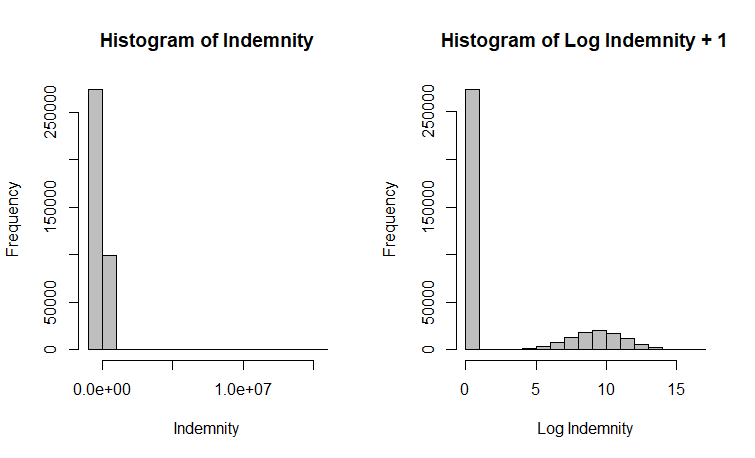
\includegraphics[width=10cm]{YumaImages/HistogramIndemnityAndLogIndemnity.png}\end{center}
\end{frame}
% Based on the table from the previous slide, it's not surprising to see that a histogram of the indemnity amounts (which you can see on the left) is heavily skewed right and has a lot of mass at 0. To better capture the distribution of the data, we did a log transformation of the indemnity amounts + 1. The + 1 is necessary to consider the zero values in our modeling. From the right figure, we see a spike at 0 and there's probability mass at other positive numbers. The Poisson sum of the positive indemnities will follow a Tweedie distribution, where the aggregate loss could either be 0 or a positive number. This is an important figure because it motivates the use of the Tweedie distribution to transform the observations into residuals. More details regarding the Tweedie model will be explained further in a bit.

% Rate map in and out of sample
\begin{frame}
\frametitle{Data}
\textbf{Relativity Map in Michigan (Training and Validation Sample)}
\begin{center}
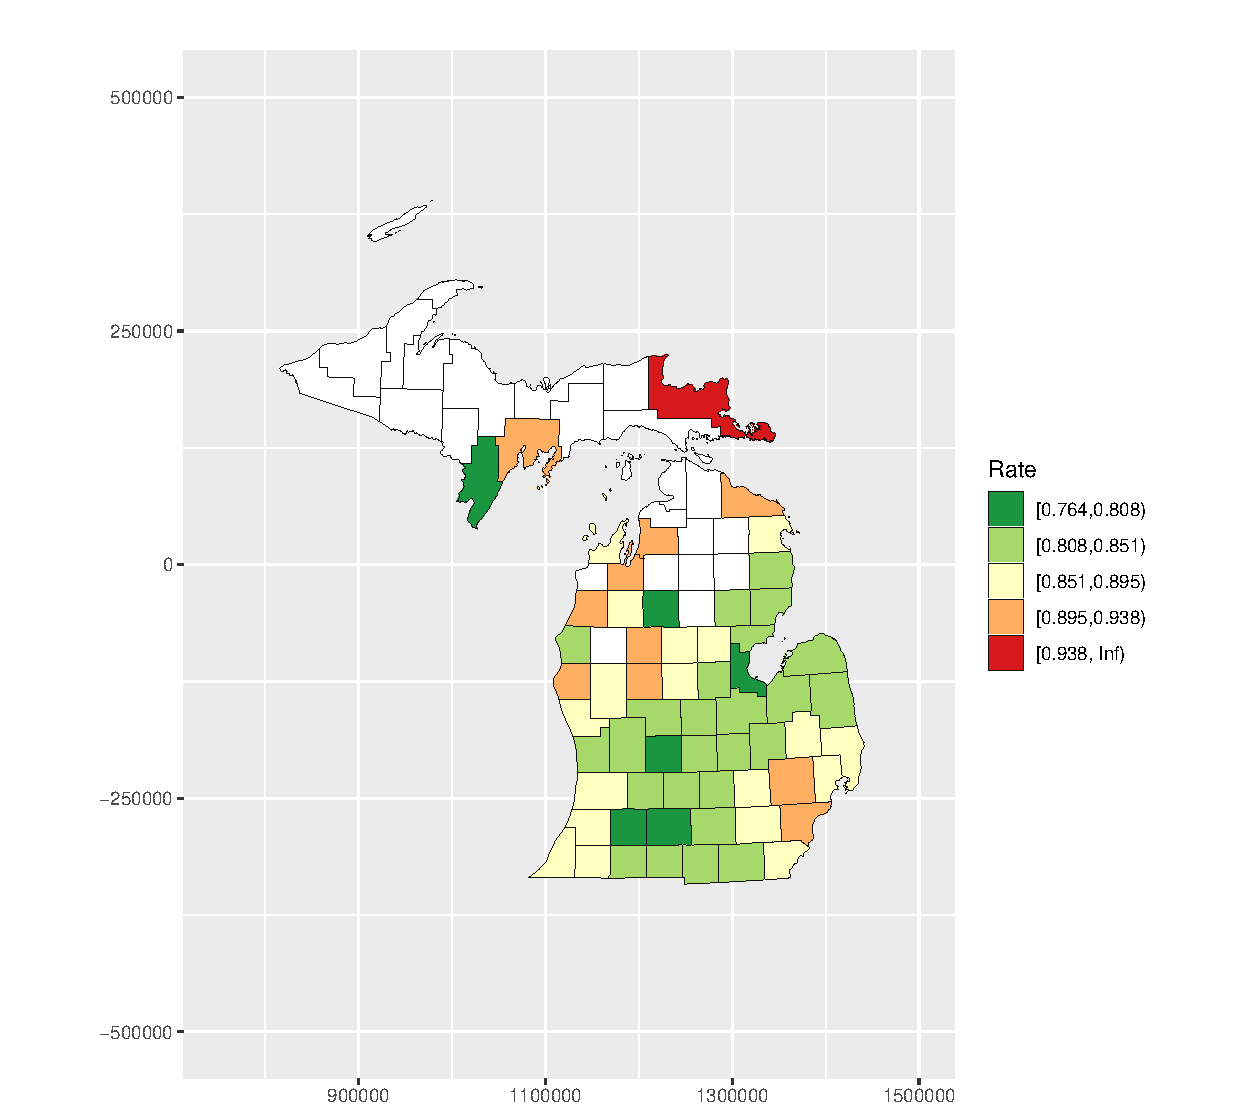
\includegraphics[width=6cm]{imgFinal/MapRateIn}
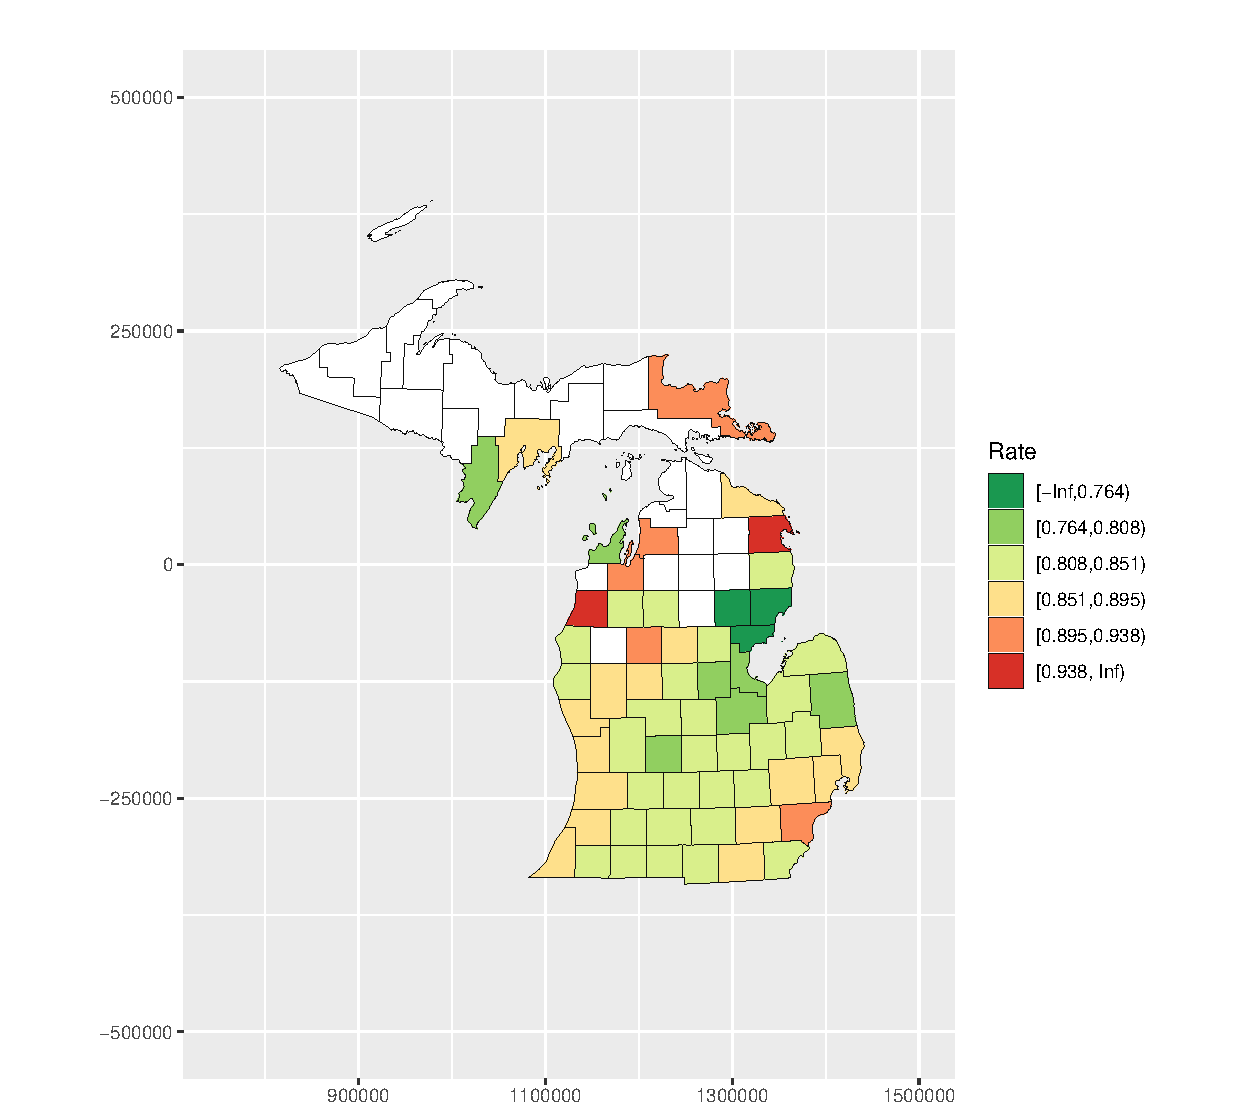
\includegraphics[width=6cm]{imgFinal/MapRateOut}\end{center}
\end{frame}
% We aggregated the indemnity amounts based on the state and county. And so we used this data as the basis for our analysis. Using Michigan as an example, the rate map on the left looks at the in-sample data, while the right figure looks at the out-of-sample data. We can visually see that the counties in which indemnity amounts were large, tend to have high indemnities in the next year as well. We see roughly the same areas highlighted in the validation sample, so there must be a lot of correlation. These figures justify the use of the in-sample data as our model for the prediction task.

% Indemnities and liabilities by peril type
\begin{frame}
\frametitle{Data}
\textbf{Indemnities and Liabilities by Peril Type}
\begin{center}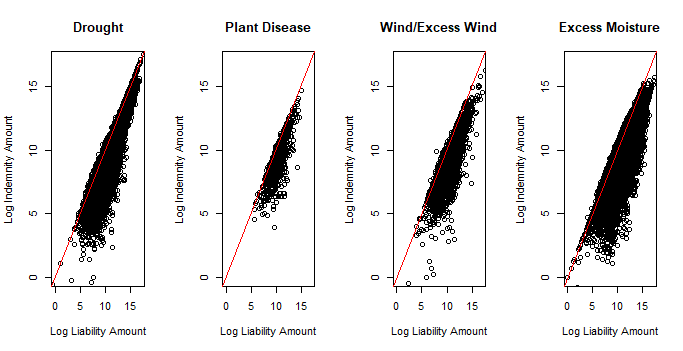
\includegraphics[width=11cm]{YumaImages/ScatterplotByPerilType.png}\end{center}
\end{frame}
% Here, we have some scatterplots of the log indemnity amount over the log liability amount for different causes of loss, like drought, plant disease, wind, and excess moisture. We can see that there's good correlation for all 4 peril types.

% Log indemnities by peril type here
\begin{frame}
\frametitle{Data}
\textbf{Log Indemnities by Peril Type}
\begin{center}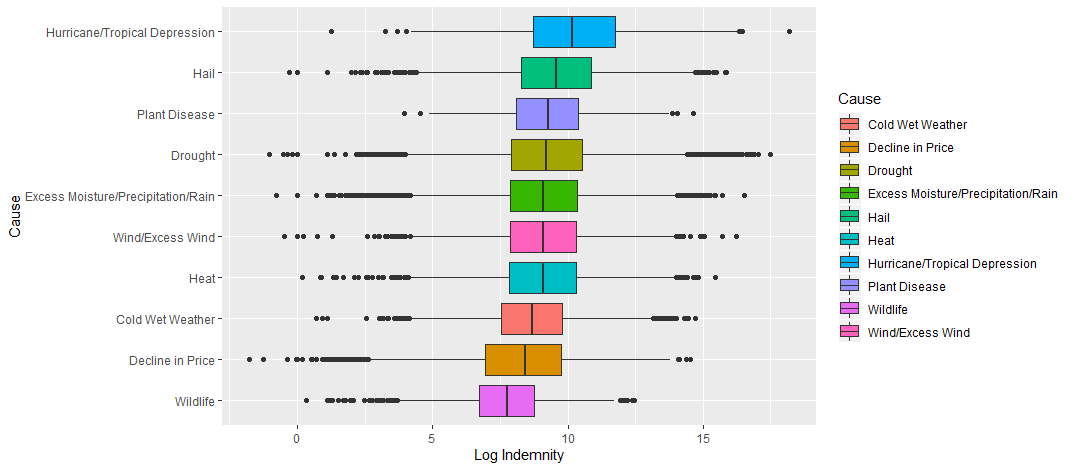
\includegraphics[width=13.5cm]{YumaImages/ByPerilType.png}\end{center}
\end{frame}
% This is a boxplot of log indemnities by peril type, where we have 10 of the most common causes of the insurance claims. We can see that hurricane/tropical depression cases had significantly different indemnity amounts compared to wildlife. This leads us to believe that each peril type has a different loss profile and also a different dependence structure.


% --------------------------------------------------------------------------------------------
\section{Analysis}
% --------------------------------------------------------------------------------------------


\begin{frame}
\frametitle{Model}
\textbf{Important Note}
\begin{itemize}
\item Most of the farms will run in the right way
\item Only a few of them will suffer a loss
\end{itemize}
\textbf{What is the Appropriate Distribution?}
\begin{itemize}
\item The answer is Tweedie Distribution
\item It is a distribution that has 0 mass and using a compound model allows us to obtain the residuals more easily
\end{itemize}
\end{frame}


\begin{frame}
\frametitle{Model}
\textbf{Introduction to Tweedie distribution}
\newline
\newline
\newline A random variable Y follows Tweedie if Y follows exponential dispersion models with mean and variance:
\begin{equation*}
	E(Y)=\mu \quad Var(Y)=\sigma^2\mu^{p}
\end{equation*}
\newline
where $p$ is called the Tweedie power parameter
\newline
\newline If $1 \leq p \leq 2 $, it will become a compound Poisson/Gamma distribution

\end{frame}


\begin{frame}
\frametitle{Model}
\textbf{Expression of Y}
\begin{equation*}
T \sim Poisson(\lambda)
\end{equation*}
\begin{equation*}
X_i \sim Gamma(\alpha,\beta)
\end{equation*}
\begin{equation*}
Y =\sum_{i=1}^{T}X_i
\end{equation*}
\textbf{Connection}

\newline The frequency of indemnity $\sim Poisson(\lambda)$
\newline The severity of indemnity $\sim Gamma(\alpha,\beta)$
\end{frame}


\begin{frame}
\frametitle{Model}
\textbf{Shape of Tweedie Distribution}
\begin{center}
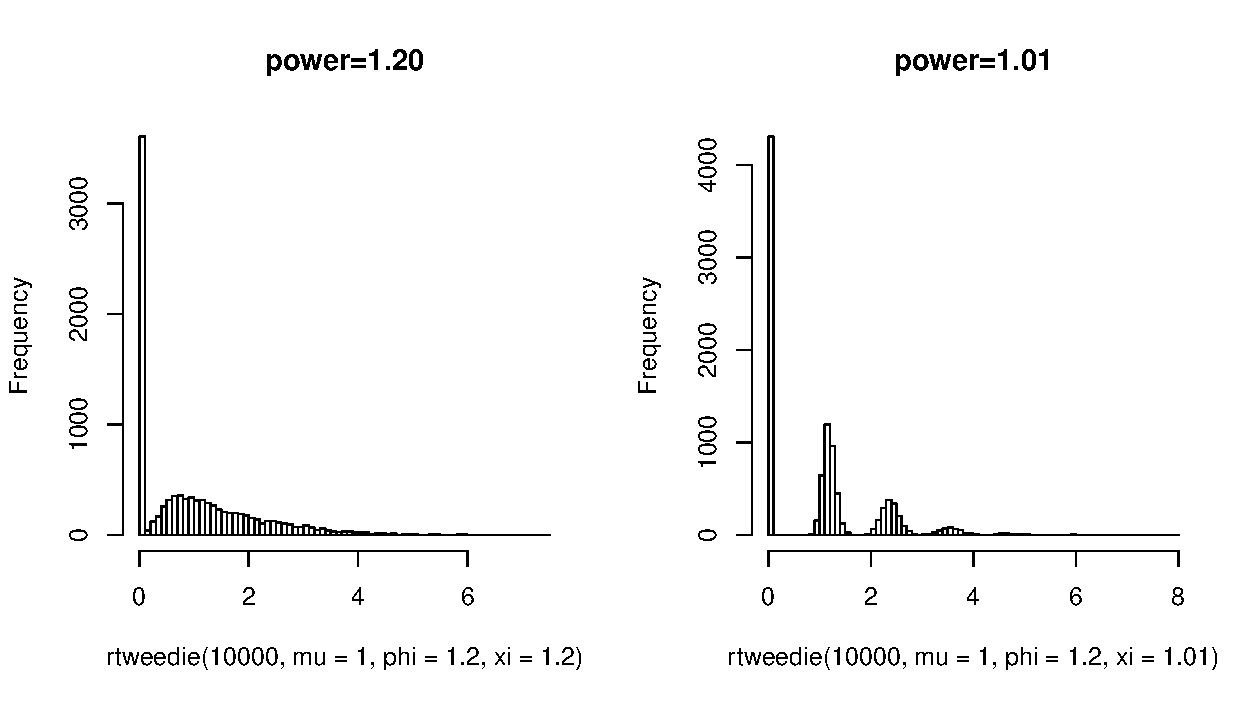
\includegraphics[width=10cm]{imgFinal/Tweedie.pdf}
\end{center}
\end{frame}

%-----------------------------------------------------------------

\begin{frame}{}
\frametitle{Model}
\textbf{Copula Function Demonstration}
\par We use the Copula function to construct three groups of data. Within each group of data, there are two normally distributed variables. The covariances in each group are 0.1, 0.9, and -0.9 respectively.
\begin{figure}

\centering
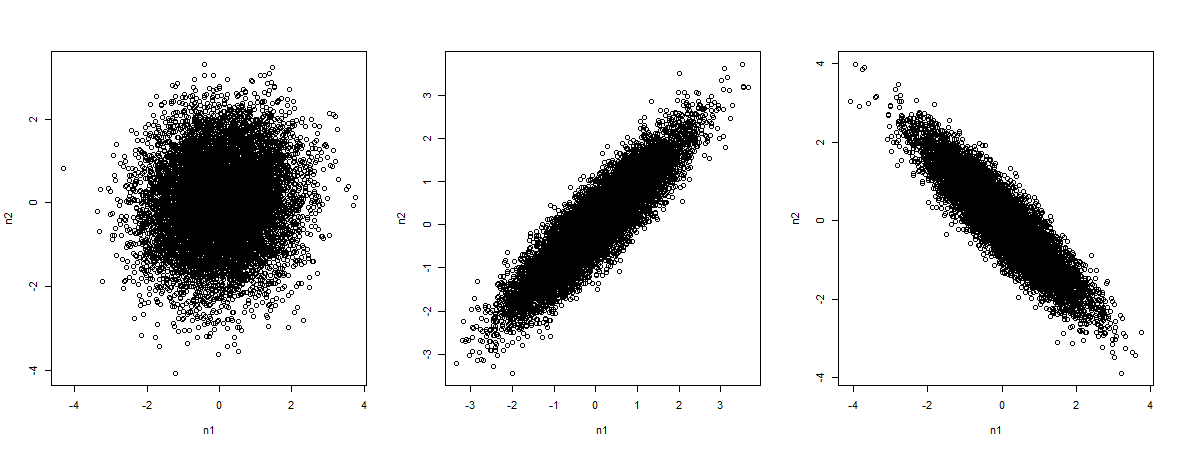
\includegraphics[scale=0.3]{1111.png}

\label{fig:pathdemo1}
\end{figure}
\begin{center}
$Var(X+Y)=Var(X)+Var(Y)+2Cov(X, Y)$
\end{center}
\end{frame}

\begin{frame}
\frametitle{Analysis}
\textbf{Some Common Peril Types}

\par (1) Drought
\par (2) Plant Disease
\par (3) Wind/Excess Wind
\par (4) Excess Moisture/Precipitation/Rain
\par (5) Hurricane/Tropical Depression

\end{frame}

\begin{frame}
\frametitle{Analysis}
\textbf{Process}
\par 
\par (1) Aggregate the information we need to generate a table
\par (2) Use the \textbf{tweedie.profile() function} to generate the \textbf{MLE} of the Tweedie index power parameter
\par (3) Construct the exact PDF of Tweedie distribution
\par (4) Obtain the Cox-Snell residuals
\par (5) Obtain the covariance

\end{frame}


\begin{frame}
\frametitle{Results}
\textbf{Covariance of Specific Peril Types}
\par 2 policyholders in the same state have correlations of:
\begin{center}
\par 
\begin{tabular}{||c|c|c|c|c||}
\hline
\textbf{Drought}& \textbf{Plant Disease}& \textbf{Wind} & \textbf{Precipitation} & \textbf{Hurricane}\\
\hline \hline
0.4581&  0.3214& 0.3116 & 0.3406 & 0.0472\\
\hline
\end{tabular}
\end{center}
\begin{itemize}
    \item Covariances indicate dependence for those policyholders within the same state
\end{itemize}
\end{frame}

\begin{frame}
\frametitle{Conclusion}
\textbf{Implications}
\begin{itemize}
    \item Different peril types have different dependence structure
    \item The risk capital held by an insurance company should be different depending on the peril types being covered
    \item Underwriting strategies and loss reserving practices may be influenced by this
\end{itemize}
\end{frame}


\begin{frame}
\Huge{\centerline{Thank you!}}
\end{frame}



\end{document}













